% 	Name		:: 	sthlm Beamer Theme  HEAVILY based on the hsrmbeamer theme (Benjamin Weiss)
%	Author		:: 	Mark Hendry Olson (mark@hendryolson.com)
%	Created		::	2013-07-31
%	Updated		::	June 18, 2015 at 08:45
%	Version		:: 	1.0.2
%	Email		:: 	hendryolson@gmail.com
%	Website		:: 	http://v42.com
%
% 	License		:: 	This file may be distributed and/or modified under the
%                  	GNU Public License.
%
%	Description	::	This presentation is a demonstration of the sthlm beamer
%					theme, which is HEAVILY based on the HSRM beamer theme created by Benjamin Weiss
%					(benjamin.weiss@student.hs-rm.de), which can be found on GitHub
%					<https://github.com/hsrmbeamertheme/hsrmbeamertheme>.


%-=-=-=-=-=-=-=-=-=-=-=-=-=-=-=-=-=-=-=-=-=-=-=-=
%
%        LOADING DOCUMENT
%
%-=-=-=-=-=-=-=-=-=-=-=-=-=-=-=-=-=-=-=-=-=-=-=-=

\documentclass[newPxFont]{beamer}
\usetheme{sthlm}
%\usecolortheme{sthlmv42}

%-=-=-=-=-=-=-=-=-=-=-=-=-=-=-=-=-=-=-=-=-=-=-=-=
%        LOADING PACKAGES
%-=-=-=-=-=-=-=-=-=-=-=-=-=-=-=-=-=-=-=-=-=-=-=-=
\usepackage[utf8]{inputenc}
\usepackage[T1]{fontenc}

%\usepackage{chronology}
\usepackage{chronosys}
\usepackage{subfigure}

\newcommand{\tabitem}{%
  \usebeamertemplate{itemize item}\hspace*{\labelsep}}


%\renewcommand{\event}[3][e]{%
%  \pgfmathsetlength\xstop{(#2-\theyearstart)*\unit}%
%  \ifx #1e%
%    \draw[fill=black,draw=none,opacity=0.5]%
%      (\xstop, 0) circle (.2\unit)%
%      node[opacity=1,rotate=45,right=.2\unit] {#3};%
%  \else%
%    \pgfmathsetlength\xstart{(#1-\theyearstart)*\unit}%
%    \draw[fill=black,draw=none,opacity=0.5,rounded corners=.1\unit]%
%      (\xstart,-.1\unit) rectangle%
%      node[opacity=1,rotate=45,right=.2\unit] {#3} (\xstop,.1\unit);%
%  \fi}%

%-=-=-=-=-=-=-=-=-=-=-=-=-=-=-=-=-=-=-=-=-=-=-=-=
%        BEAMER OPTIONS
%-=-=-=-=-=-=-=-=-=-=-=-=-=-=-=-=-=-=-=-=-=-=-=-=

%\setbeameroption{show notes}

%-=-=-=-=-=-=-=-=-=-=-=-=-=-=-=-=-=-=-=-=-=-=-=-=
%
%	PRESENTATION INFORMATION
%
%-=-=-=-=-=-=-=-=-=-=-=-=-=-=-=-=-=-=-=-=-=-=-=-=

\title{ComExp}
\subtitle{Comment pousser l'accompagnement jusqu'a l'exploration des modèles a base d'agents.}
%\date{\small{\jobname}}
%\date{\today}
\author{\texttt{E. Delay}\\
avec une aimable stimulation de \texttt{R. Reuillon}, \texttt{P. Chapron} et \texttt{M. Leclaire}}
\institute{CIRAD -- UMR SENS}

\hypersetup{
pdfauthor = {E. DELAY},
pdfsubject = {Seminaire SENS},
pdfkeywords = {Communs, Simulation, solidarité},
pdfmoddate= {\pdfdate},
pdfcreator = {}
}

\begin{document}

%-=-=-=-=-=-=-=-=-=-=-=-=-=-=-=-=-=-=-=-=-=-=-=-=
%
%	TITLE PAGE
%
%-=-=-=-=-=-=-=-=-=-=-=-=-=-=-=-=-=-=-=-=-=-=-=-=


\maketitle

%\begin{frame}[plain]
%	\titlepage
%\end{frame}

%-=-=-=-=-=-=-=-=-=-=-=-=-=-=-=-=-=-=-=-=-=-=-=-=
%
%	TABLE OF CONTENTS: OVERVIEW
%
%-=-=-=-=-=-=-=-=-=-=-=-=-=-=-=-=-=-=-=-=-=-=-=-=
% \section*{Une boussole ?}
% \begin{frame}{Overview}
% % For longer presentations use hideallsubsections option
% \tableofcontents[hideallsubsections]
% \end{frame}

%-=-=-=-=-=-=-=-=-=-=-=-=-=-=-=-=-=-=-=-=-=-=-=-=
%	FRAME: INTRODUCTION
%-=-=-=-=-=-=-=-=-=-=-=-=-=-=-=-=-=-=-=-=-=-=-=-=

\section{Introduction :\\ au commencement il y avait ComMod}
  \begin{frame}[c]{L'Egalité comme prérequis}
    \vspace{-1cm}
    \begin{columns}[onlytextwidth,T]
      \column{\dimexpr\linewidth-30mm-5mm}
          \begin{itemize}
            \item Le \textit{``maître ignorant''} de Rancière (2003) qui accompagne : <<\emph{contrairement à ce que laissent penser nos positions sociales, nous sommes égaux, voyons ce que nous pouvons en faire}>>
            \item Le diplomate de Morizot (2020) cherche les axes de mobilisation, car <<\emph{une fois qu’on a circulé parmi les points de vue, on sent que certains n’ont pas la légitimité qu’ils réclament.}>>
          \end{itemize}

          \small{
              \begin{alertblock}{\textsc{Une posture philosophique}}
                Entre \textsc{Rancière} et \textsc{Morizot}, on a les composantes de la posture des acteurs du vivre ensemble.
              \end{alertblock}
            }
      \column{30mm}
      \vspace{0.5cm}
            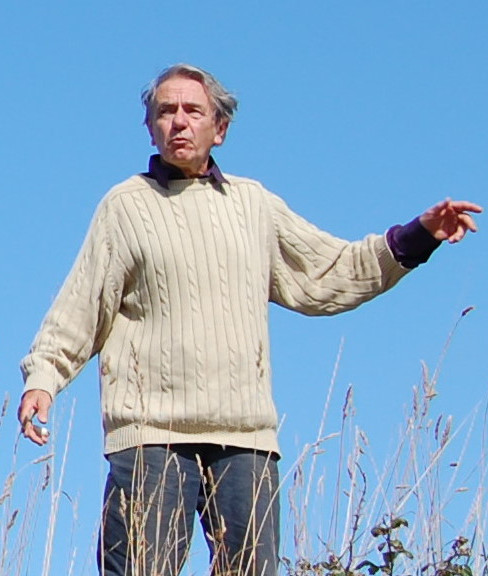
\includegraphics[width=3cm]{img/Ranciere.jpg}\\
            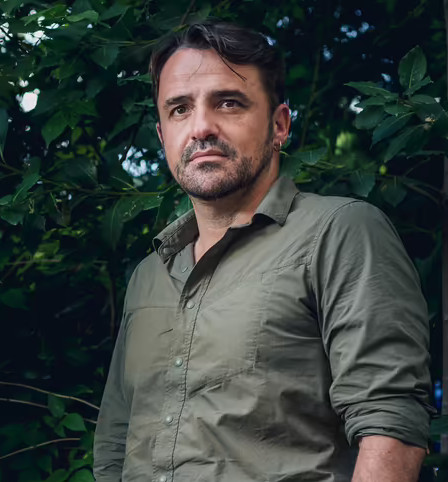
\includegraphics[width=3cm]{img/morizot.jpg}
    \end{columns}
  \end{frame}

  \begin{frame}[c]{L'Equité : un objectif ?}
    \vspace{-1cm}
    l'approche par les communs a besoin d'un préalable, qui est l'égalité entre les participants.
    \begin{figure}
      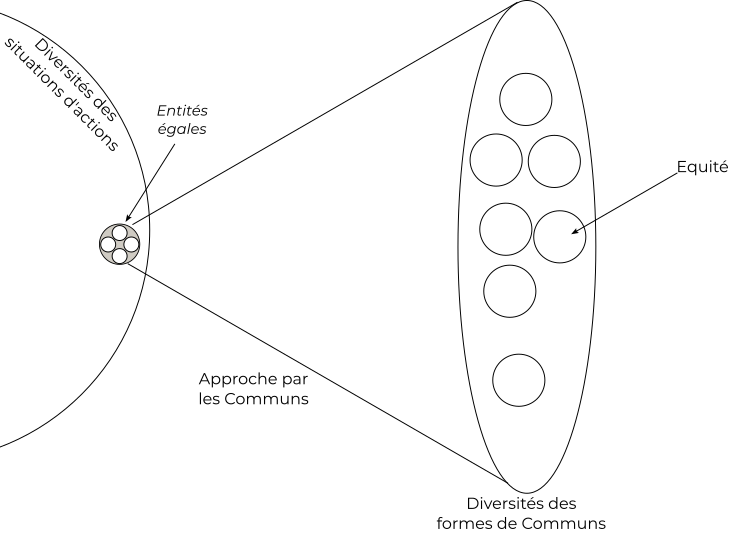
\includegraphics[height=7cm]{img/commun_egalite_equite.png}
    \end{figure}
  \end{frame}

  \begin{frame}[c]{Le decalage prometheen et l'urgence environnementale}
    \vspace{-1cm}
    \begin{columns}[onlytextwidth,T]
      \column{\dimexpr\linewidth-30mm-5mm}
      \begin{itemize}
        \item Dans \textit{"l'obsolescence de l'Homme"} Günther Anders (1956) propose la notion de décalage prométhéen,
        \item c'est-à-dire le fait que les capacités de fabrication dépassent de très loin nos possibilités de représentation
      \end{itemize}

      \small{
        \begin{alertblock}{\textsc{Une hypothese forte}}
          Accompagner les participants, c'est réduire le décalage prométhéen, et permettre le passage à l'action.
        \end{alertblock}
      }
      \column{30mm}
      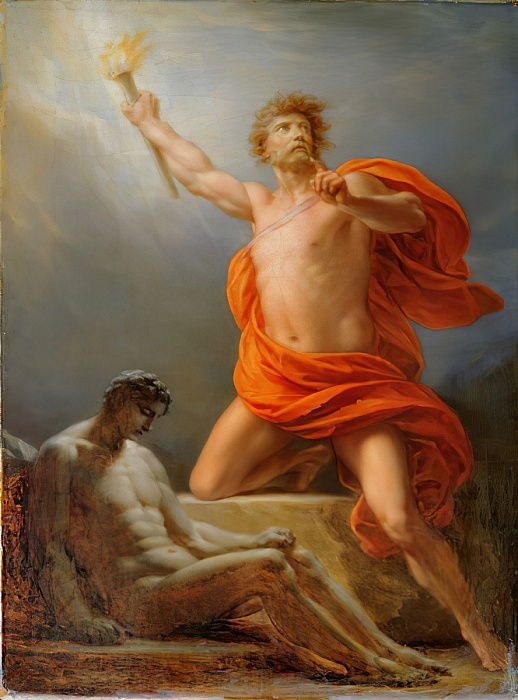
\includegraphics[height=5cm]{img/promethee.jpg}
    \end{columns}
  \end{frame}

%-=-=-=-=-=-=-=-=-=-=-=-=-=-=-=-=-=-=-=-=-=-=-=-=
%	FRAME: ComExp qu'est-ce que c'est ? 
%-=-=-=-=-=-=-=-=-=-=-=-=-=-=-=-=-=-=-=-=-=-=-=-=

\section{ComExp\\ Un etage de plus a la fuse ComMod}


\begin{frame}[c]{ComExp c'est ComMod}
  \vspace{-1cm}
  Avec des ateliers de co-construction
  \begin{center}
  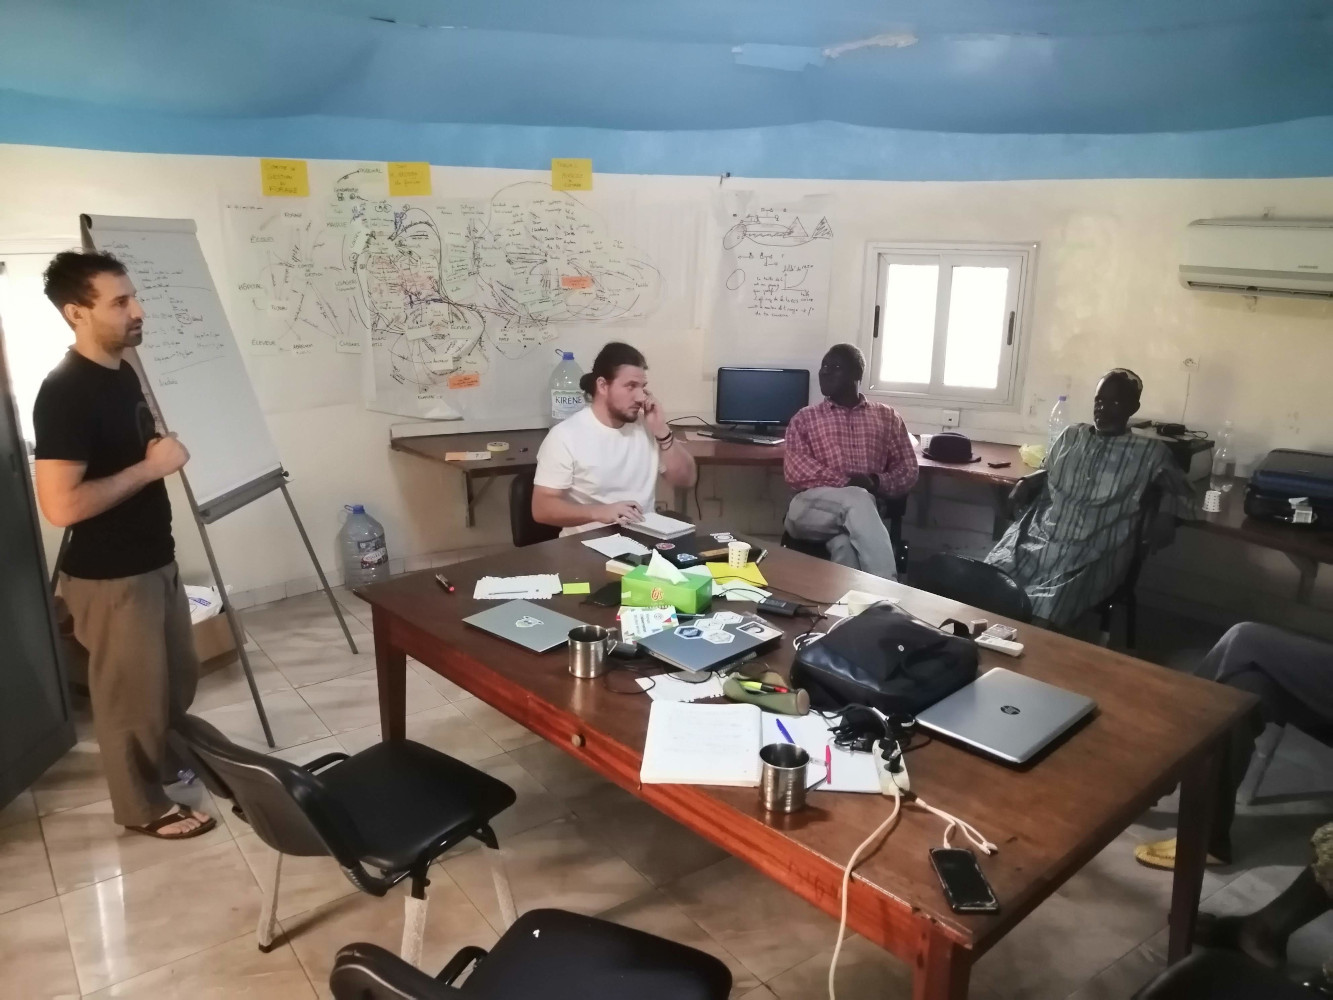
\includegraphics[width=7cm]{img/atelier_niakhar.jpg}
  \end{center}
\end{frame}

\begin{frame}[c]{ComExp c'est ComMod}
  \vspace{-1cm}
  Avec des ARDI en \texttt{.dot}
  \begin{center}
  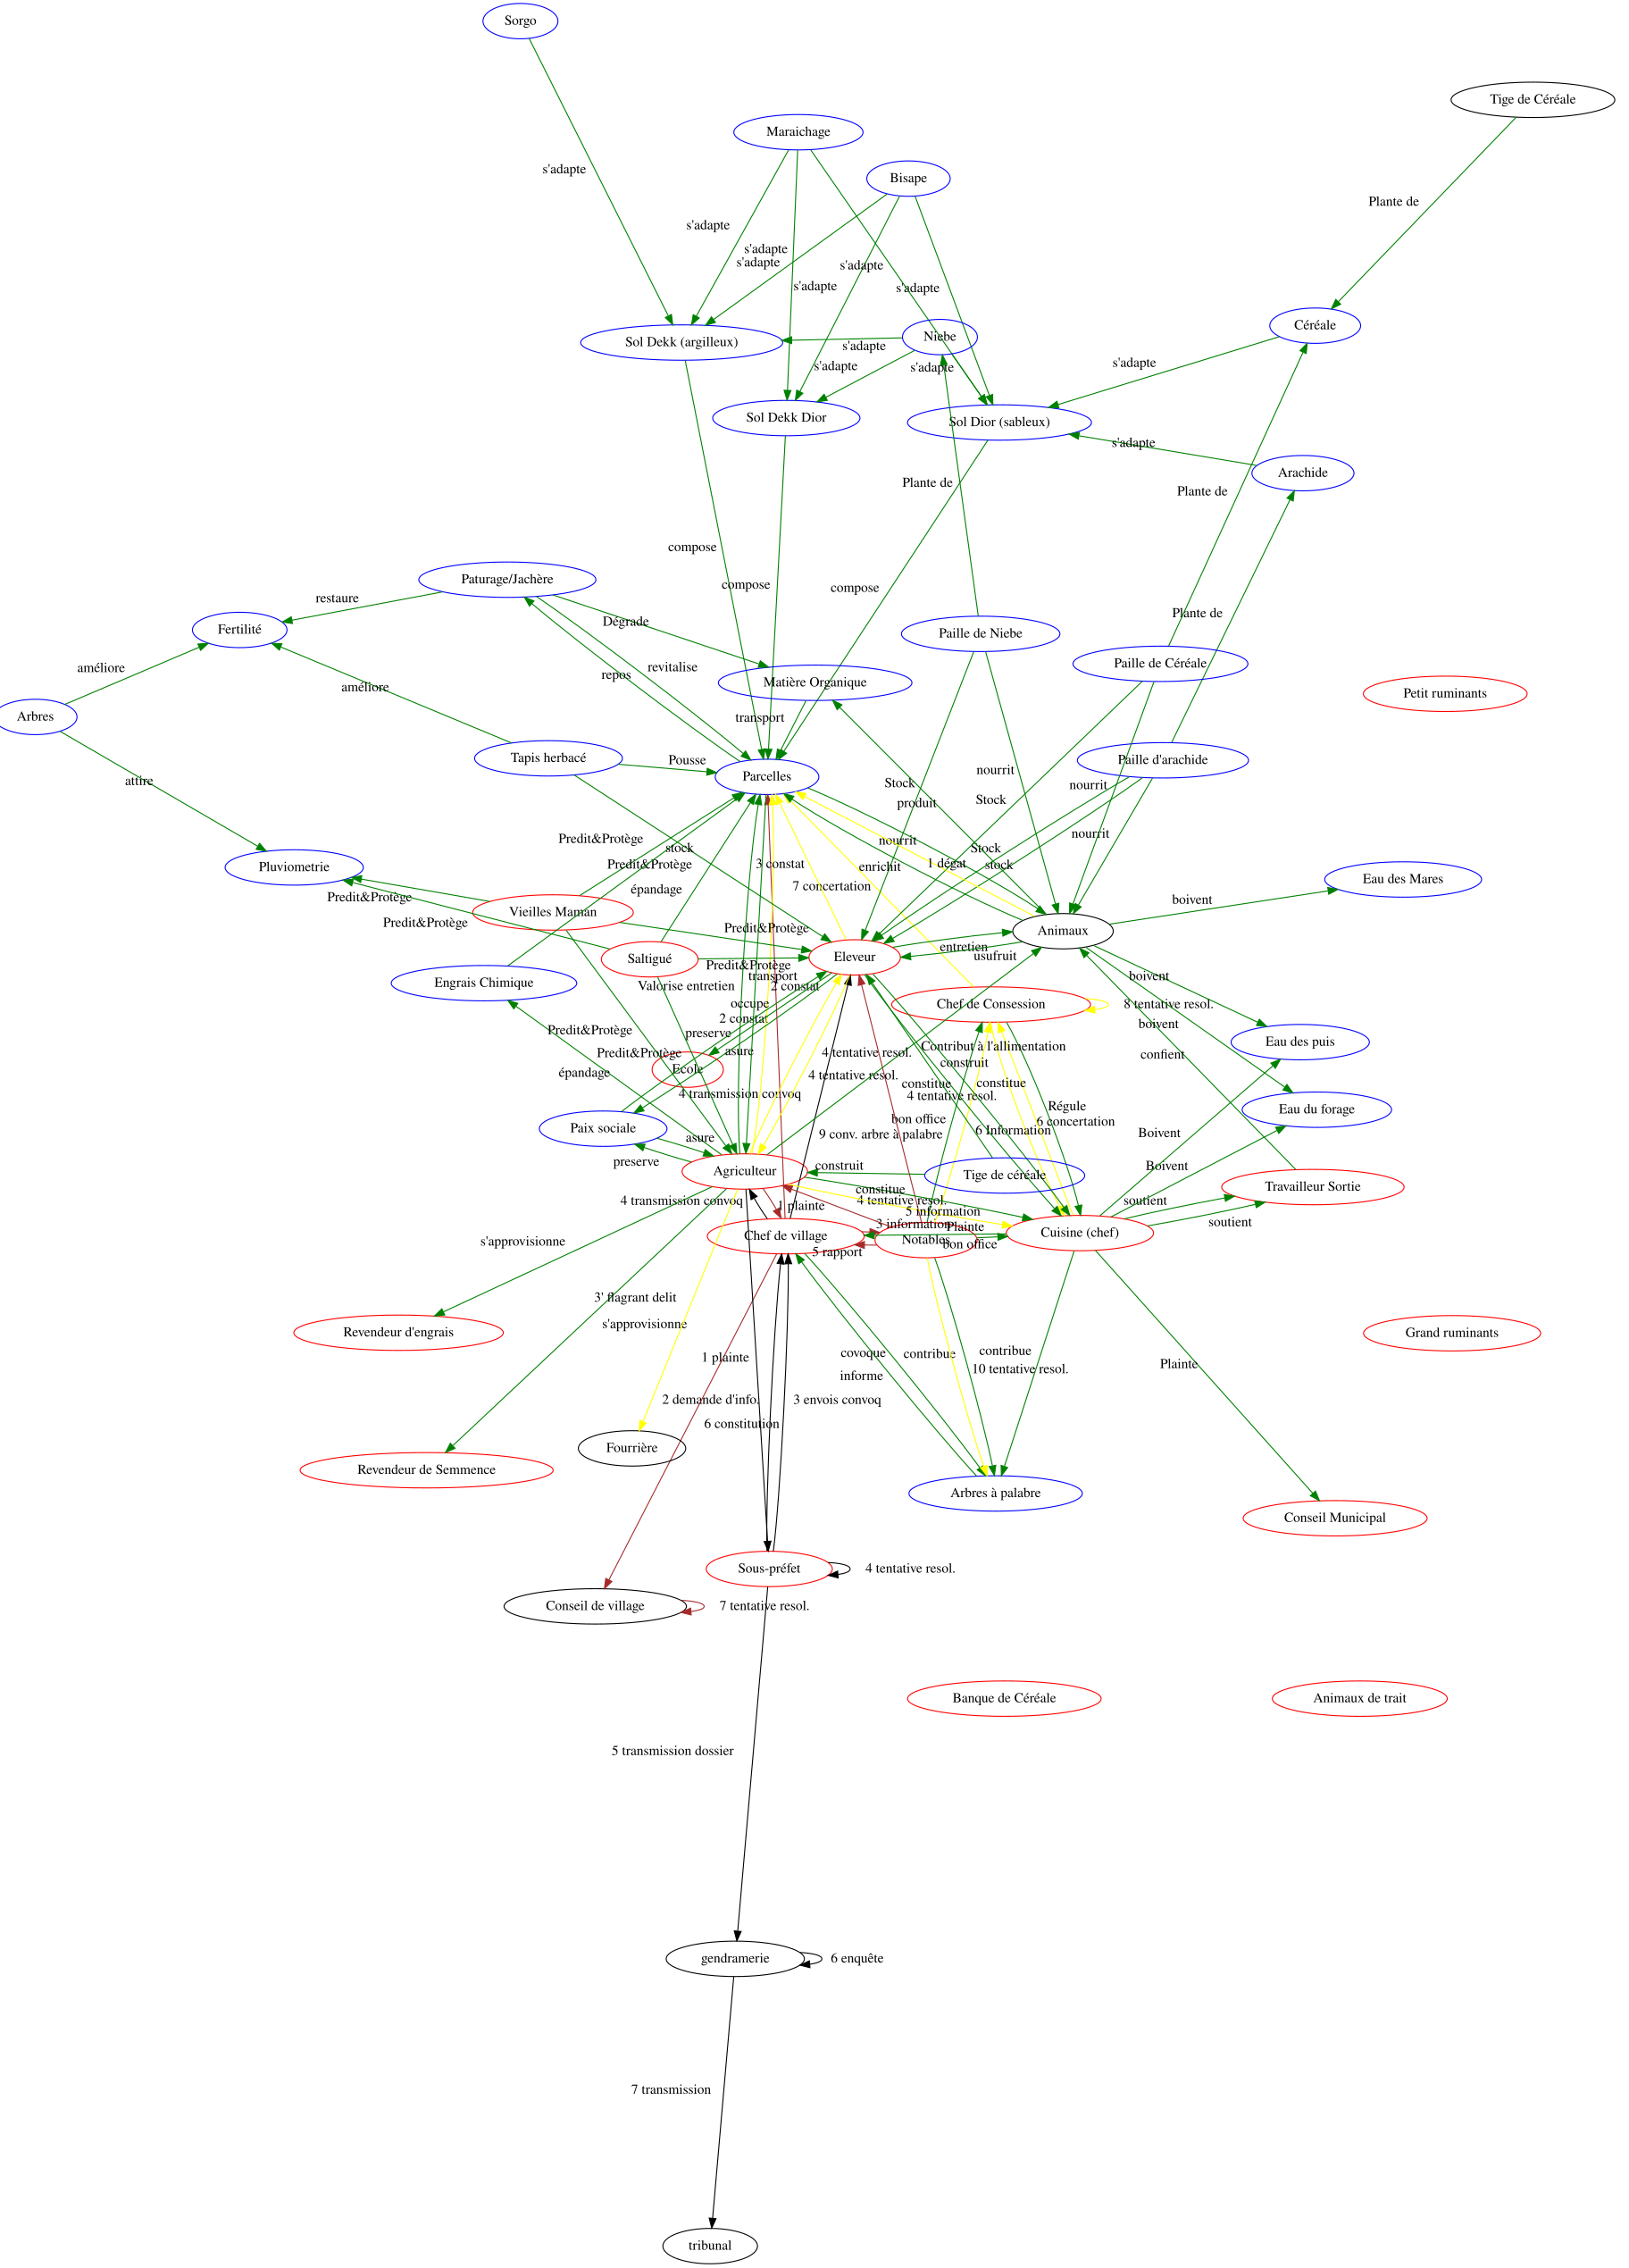
\includegraphics[width=8cm]{img/pardi_fdp.png}
  \end{center}
\end{frame}

\begin{frame}[c]{ComExp c'est ComMod}
  \vspace{-1cm}
  Avec des modèles de simulations
  \begin{center}
  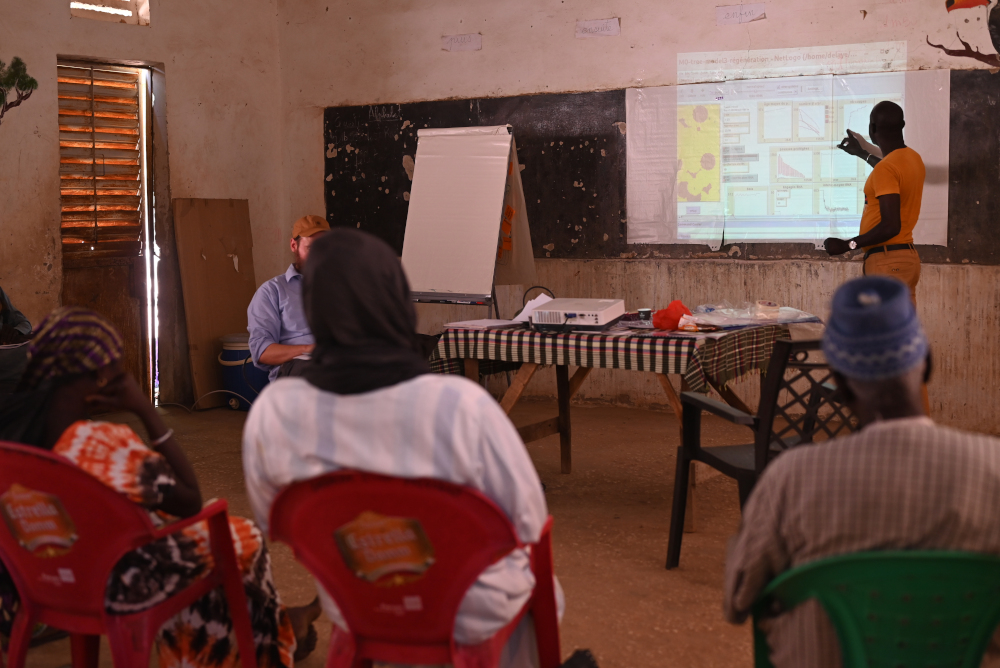
\includegraphics[width=9cm]{img/modelSimu.JPG}
  \end{center}
\end{frame}

\begin{frame}[c]{Mais ComMod, avec un petit truc en plus}
  \vspace{-1cm}
  \small Un usage massif au calcul en essayant d'échapper a la malédiction des dimensions.
\begin{center}
 %
\includegraphics[width=6cm]{img/OpenMOLE-Banner.png}\\
 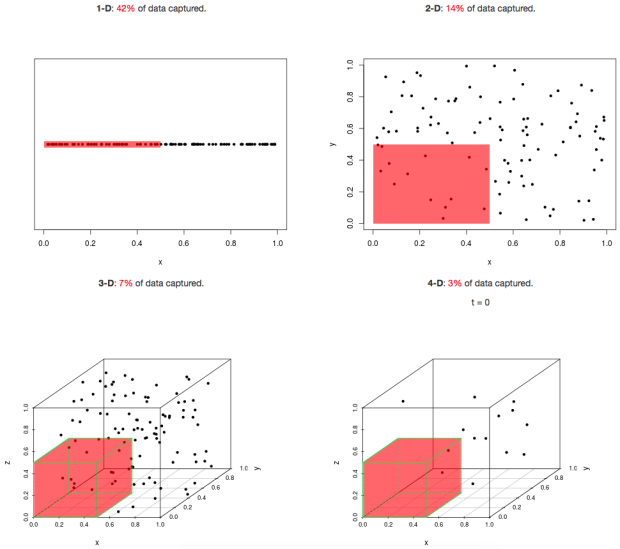
\includegraphics[width=8cm]{img/CurseOfDimensionality.png}
\end{center}
\end{frame}

%-=-=-=-=-=-=-=-=-=-=-=-=-=-=-=-=-=-=-=-=-=-=-=-=
%	FRAME: ComEXp - pour quoi faire ? 
%-=-=-=-=-=-=-=-=-=-=-=-=-=-=-=-=-=-=-=-=-=-=-=-=

\section{ComExp\\ pour quoi faire ?}

\begin{frame}[c]{Chercher les bordures}
  \vspace{-1cm}
  \begin{columns}[onlytextwidth,T]
    \column{\dimexpr\linewidth-30mm-5mm}
        \begin{itemize}
          \item Des algorythme génétiques
          \item Optimiser VS chercher la diversité
        \end{itemize}
        \begin{alertblock}{\textsc{Prendre appui pour changer}}
          C'est parce qu'on peut prendre appui sur les bords du système, rediscuter les contrôles, donner du sens aux intervention qu'on peut transformer les rapports de forces et la connaissance (F. Julien, p.15, 2009).
         \end{alertblock}
    \column{30mm}
    \vspace{0.5cm}
    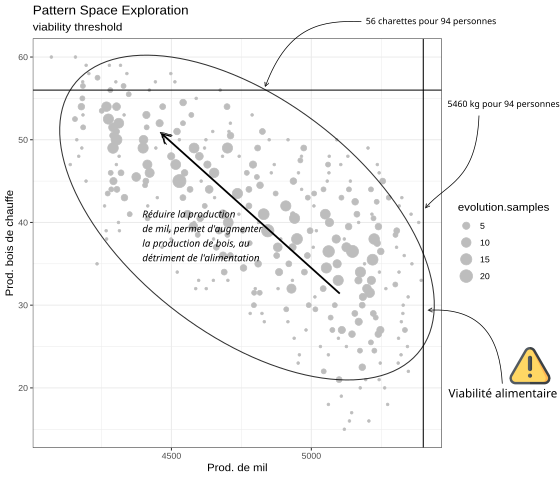
\includegraphics[width=7cm]{img/pse.png}
  \end{columns}
\end{frame}

\begin{frame}[c]{Le possible et le plausible}
  \vspace{-1cm}
  \begin{itemize}
    \item \textbf{Possible}\footnote{Définition du Centre de Ressources Textuelles et Lexicales \url{https://cnrtl.fr/definition/possible}, consulté le 11 décembre 2024.} : Adj. Qui remplit les conditions nécessaires pour être, exister, se produire sans que cela implique une réalisation effective ou que l'on sache si cette réalisation a été, est ou sera effective.

    \item \textbf{Plausible}\footnote{Définition du Centre de Ressources Textuelles et Lexicales \url{https://cnrtl.fr/definition/plausible}, consulté le 11 décembre 2024.} : Que l'on peut admettre ou croire parce que vraisemblable.
\end{itemize}
\begin{center}
 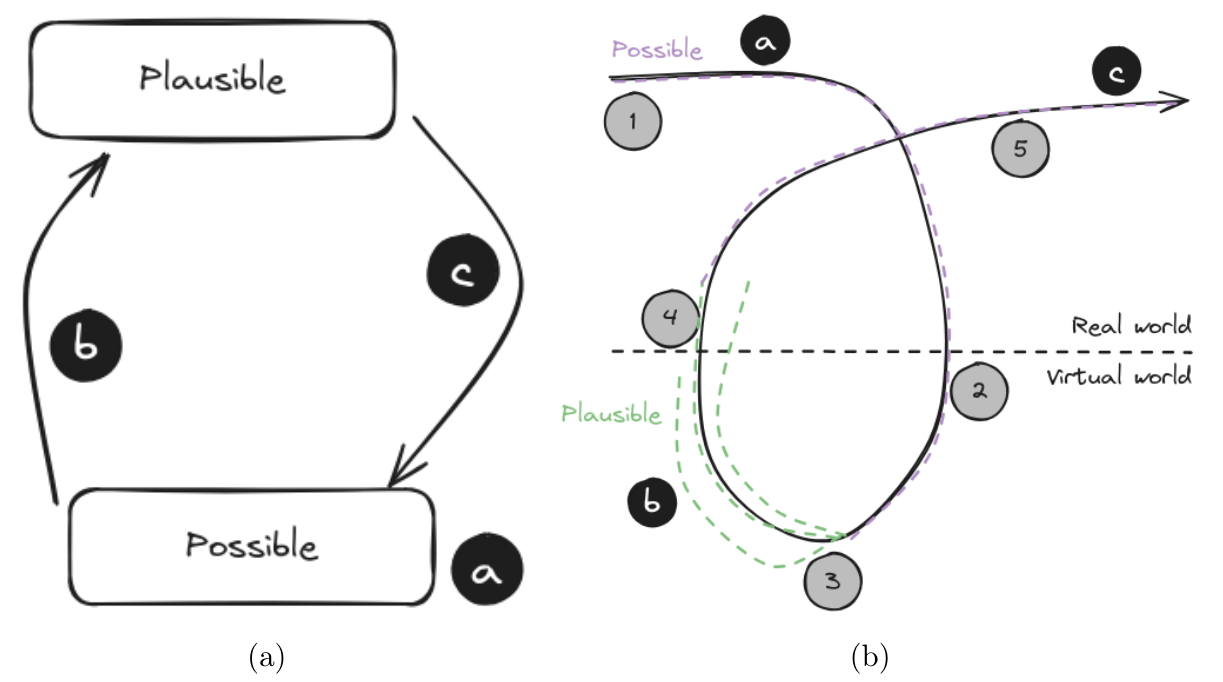
\includegraphics[width=9cm]{img/possiblePlausible.png}
\end{center}
\end{frame}

\begin{frame}[c]{Pour anticiper}
  \vspace{-1cm}
\begin{center}
  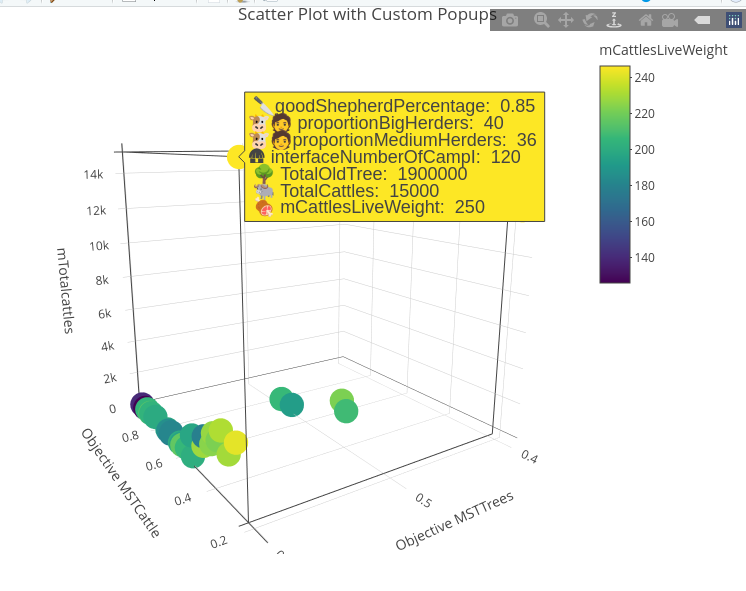
\includegraphics[width=5cm]{img/dundiModel_explo.png}
  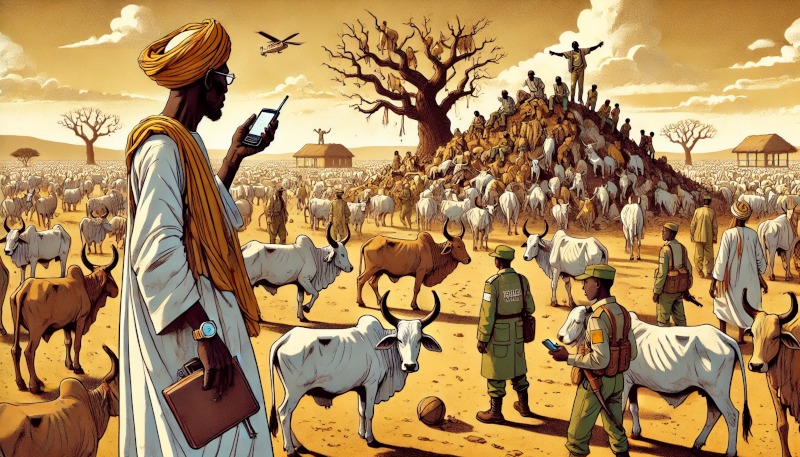
\includegraphics[width=6cm]{img/dundiModel.png}
\end{center}
\end{frame}

\begin{frame}[c]{Aller chercher le réseau soc. tech.}
  \vspace{-1cm}
\begin{center}
  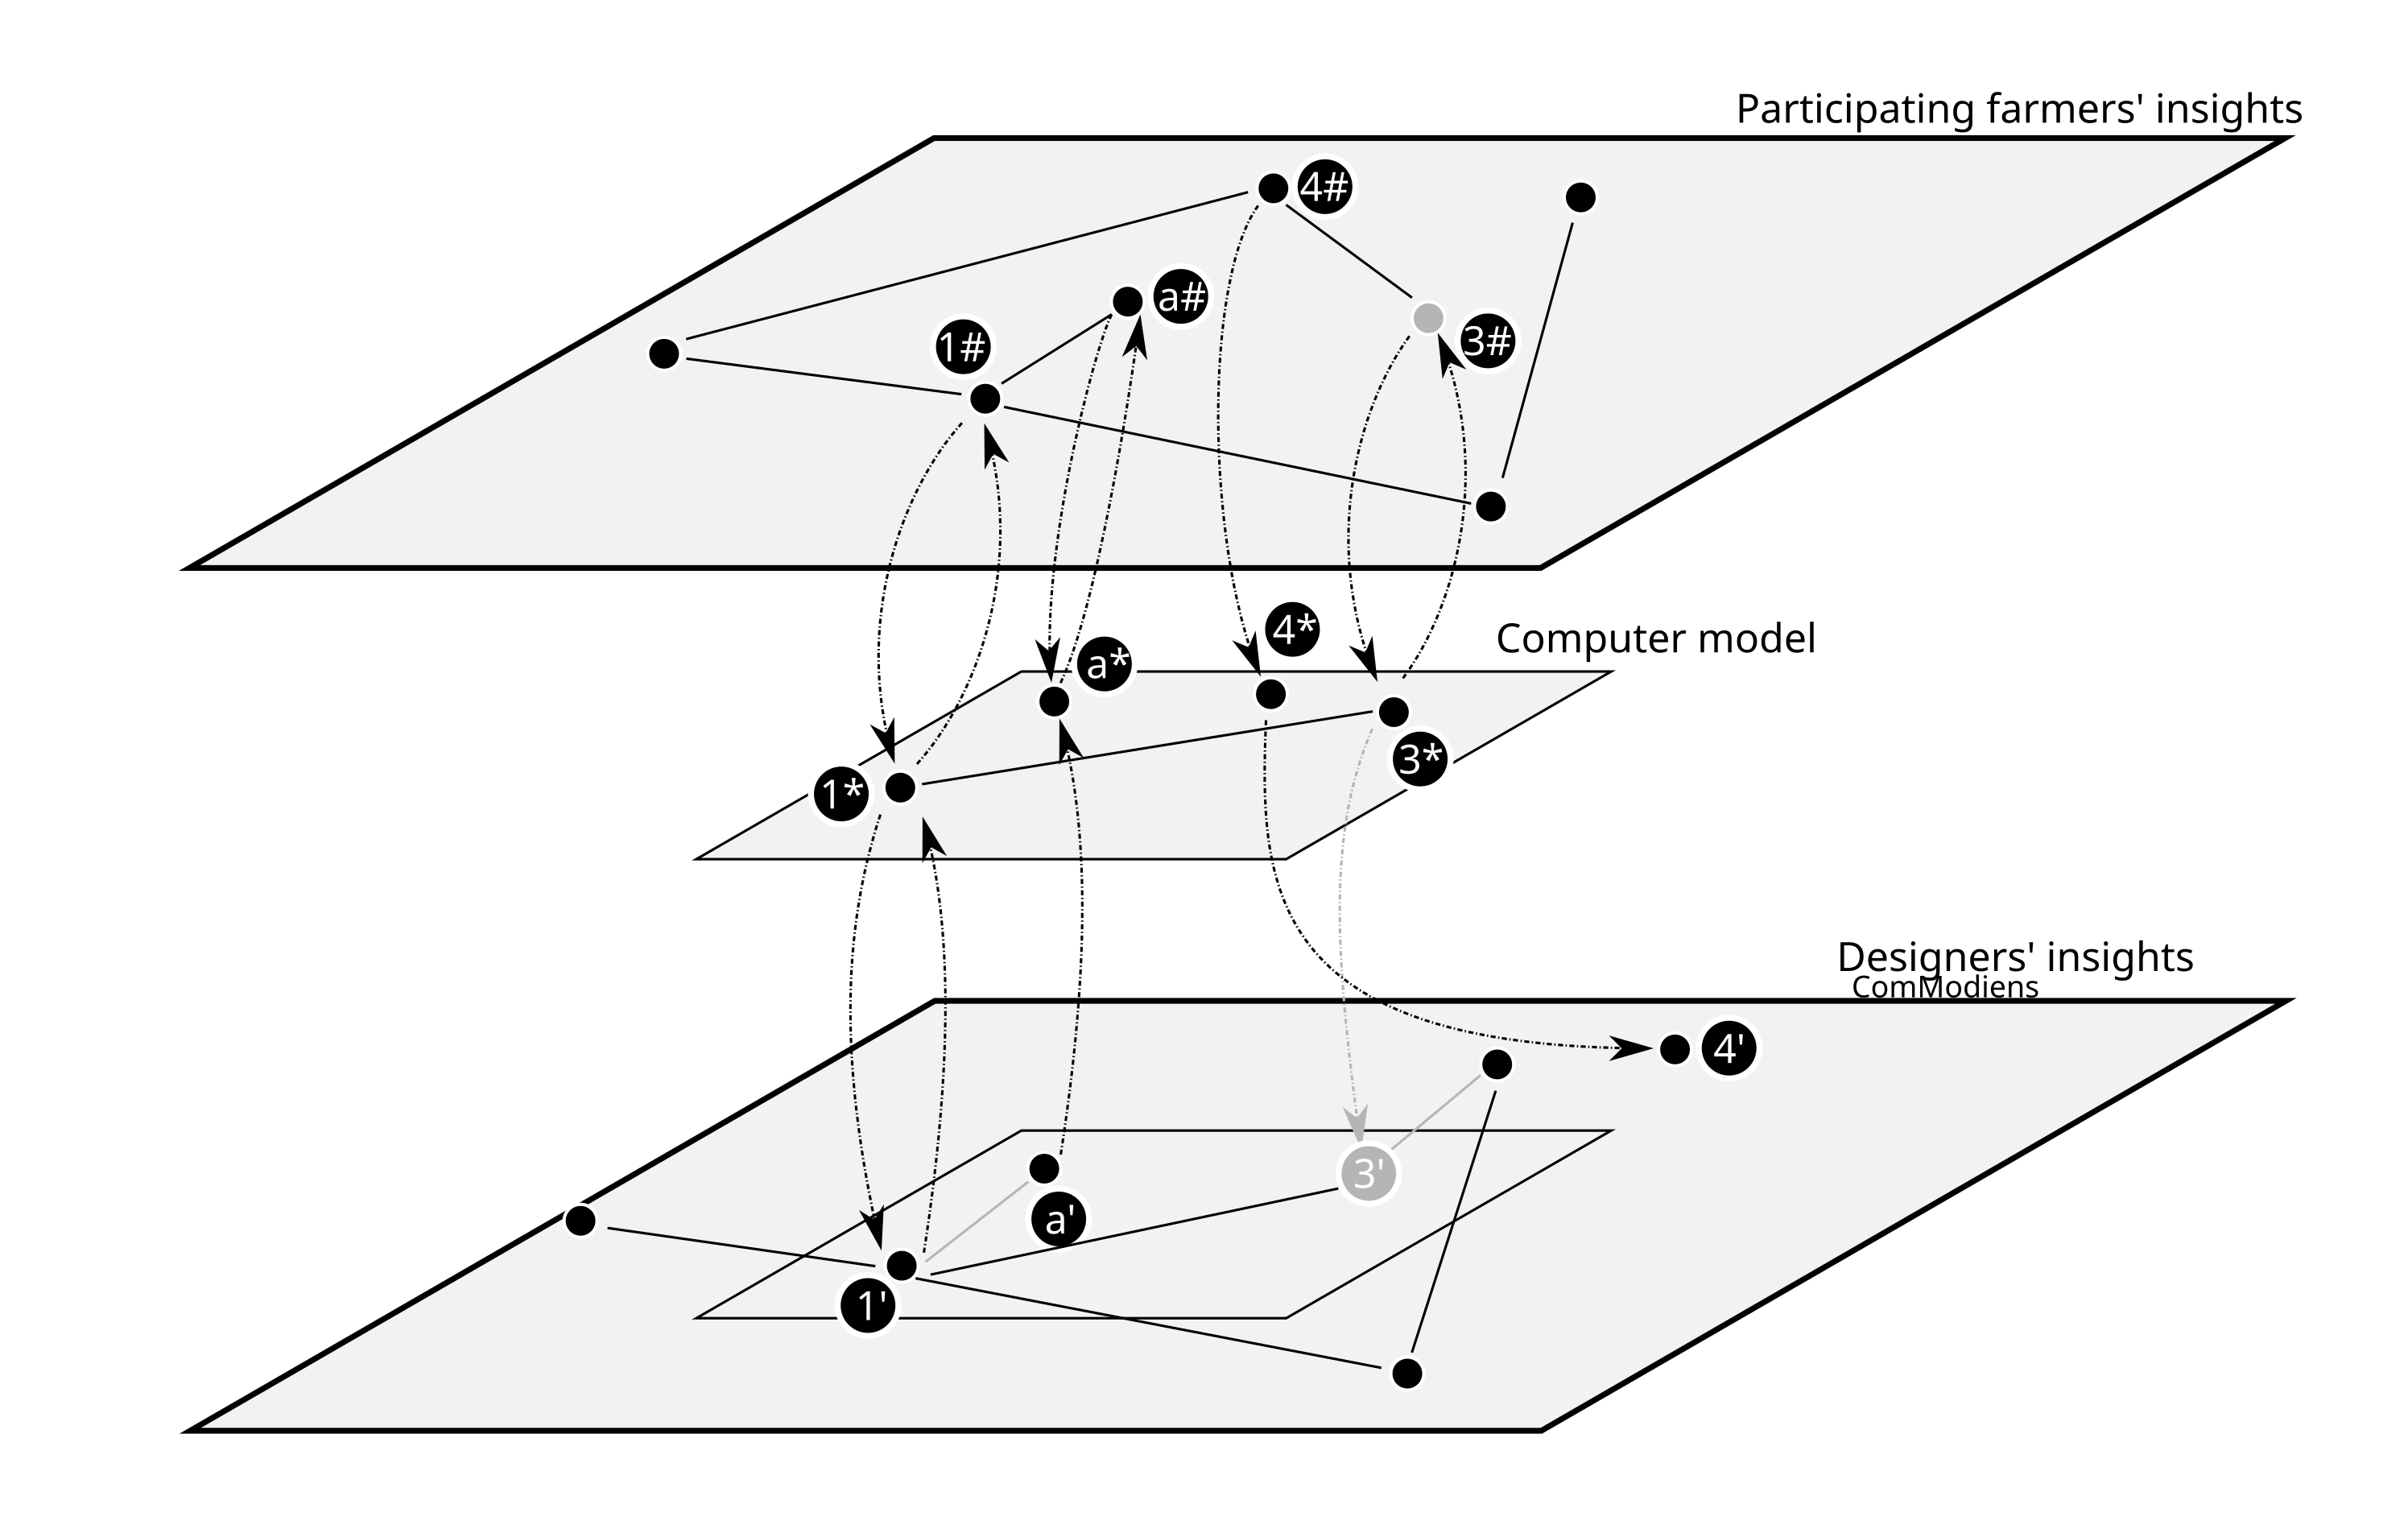
\includegraphics[width=9cm]{img/fig-construction-elements-jeu-beneficiaire_eng}
\end{center}
\end{frame}


\begin{frame}[c]{Traquer les changements de régime}
  \vspace{-1cm}
  \begin{center}
    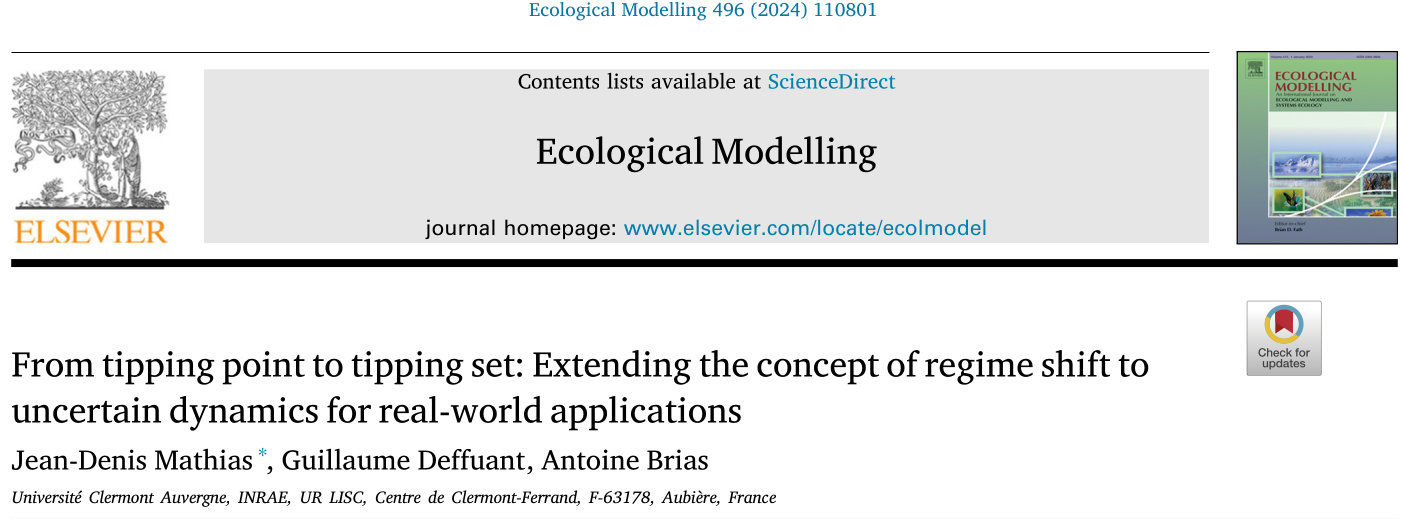
\includegraphics[width=7cm]{img/2024mathias.png}\\
    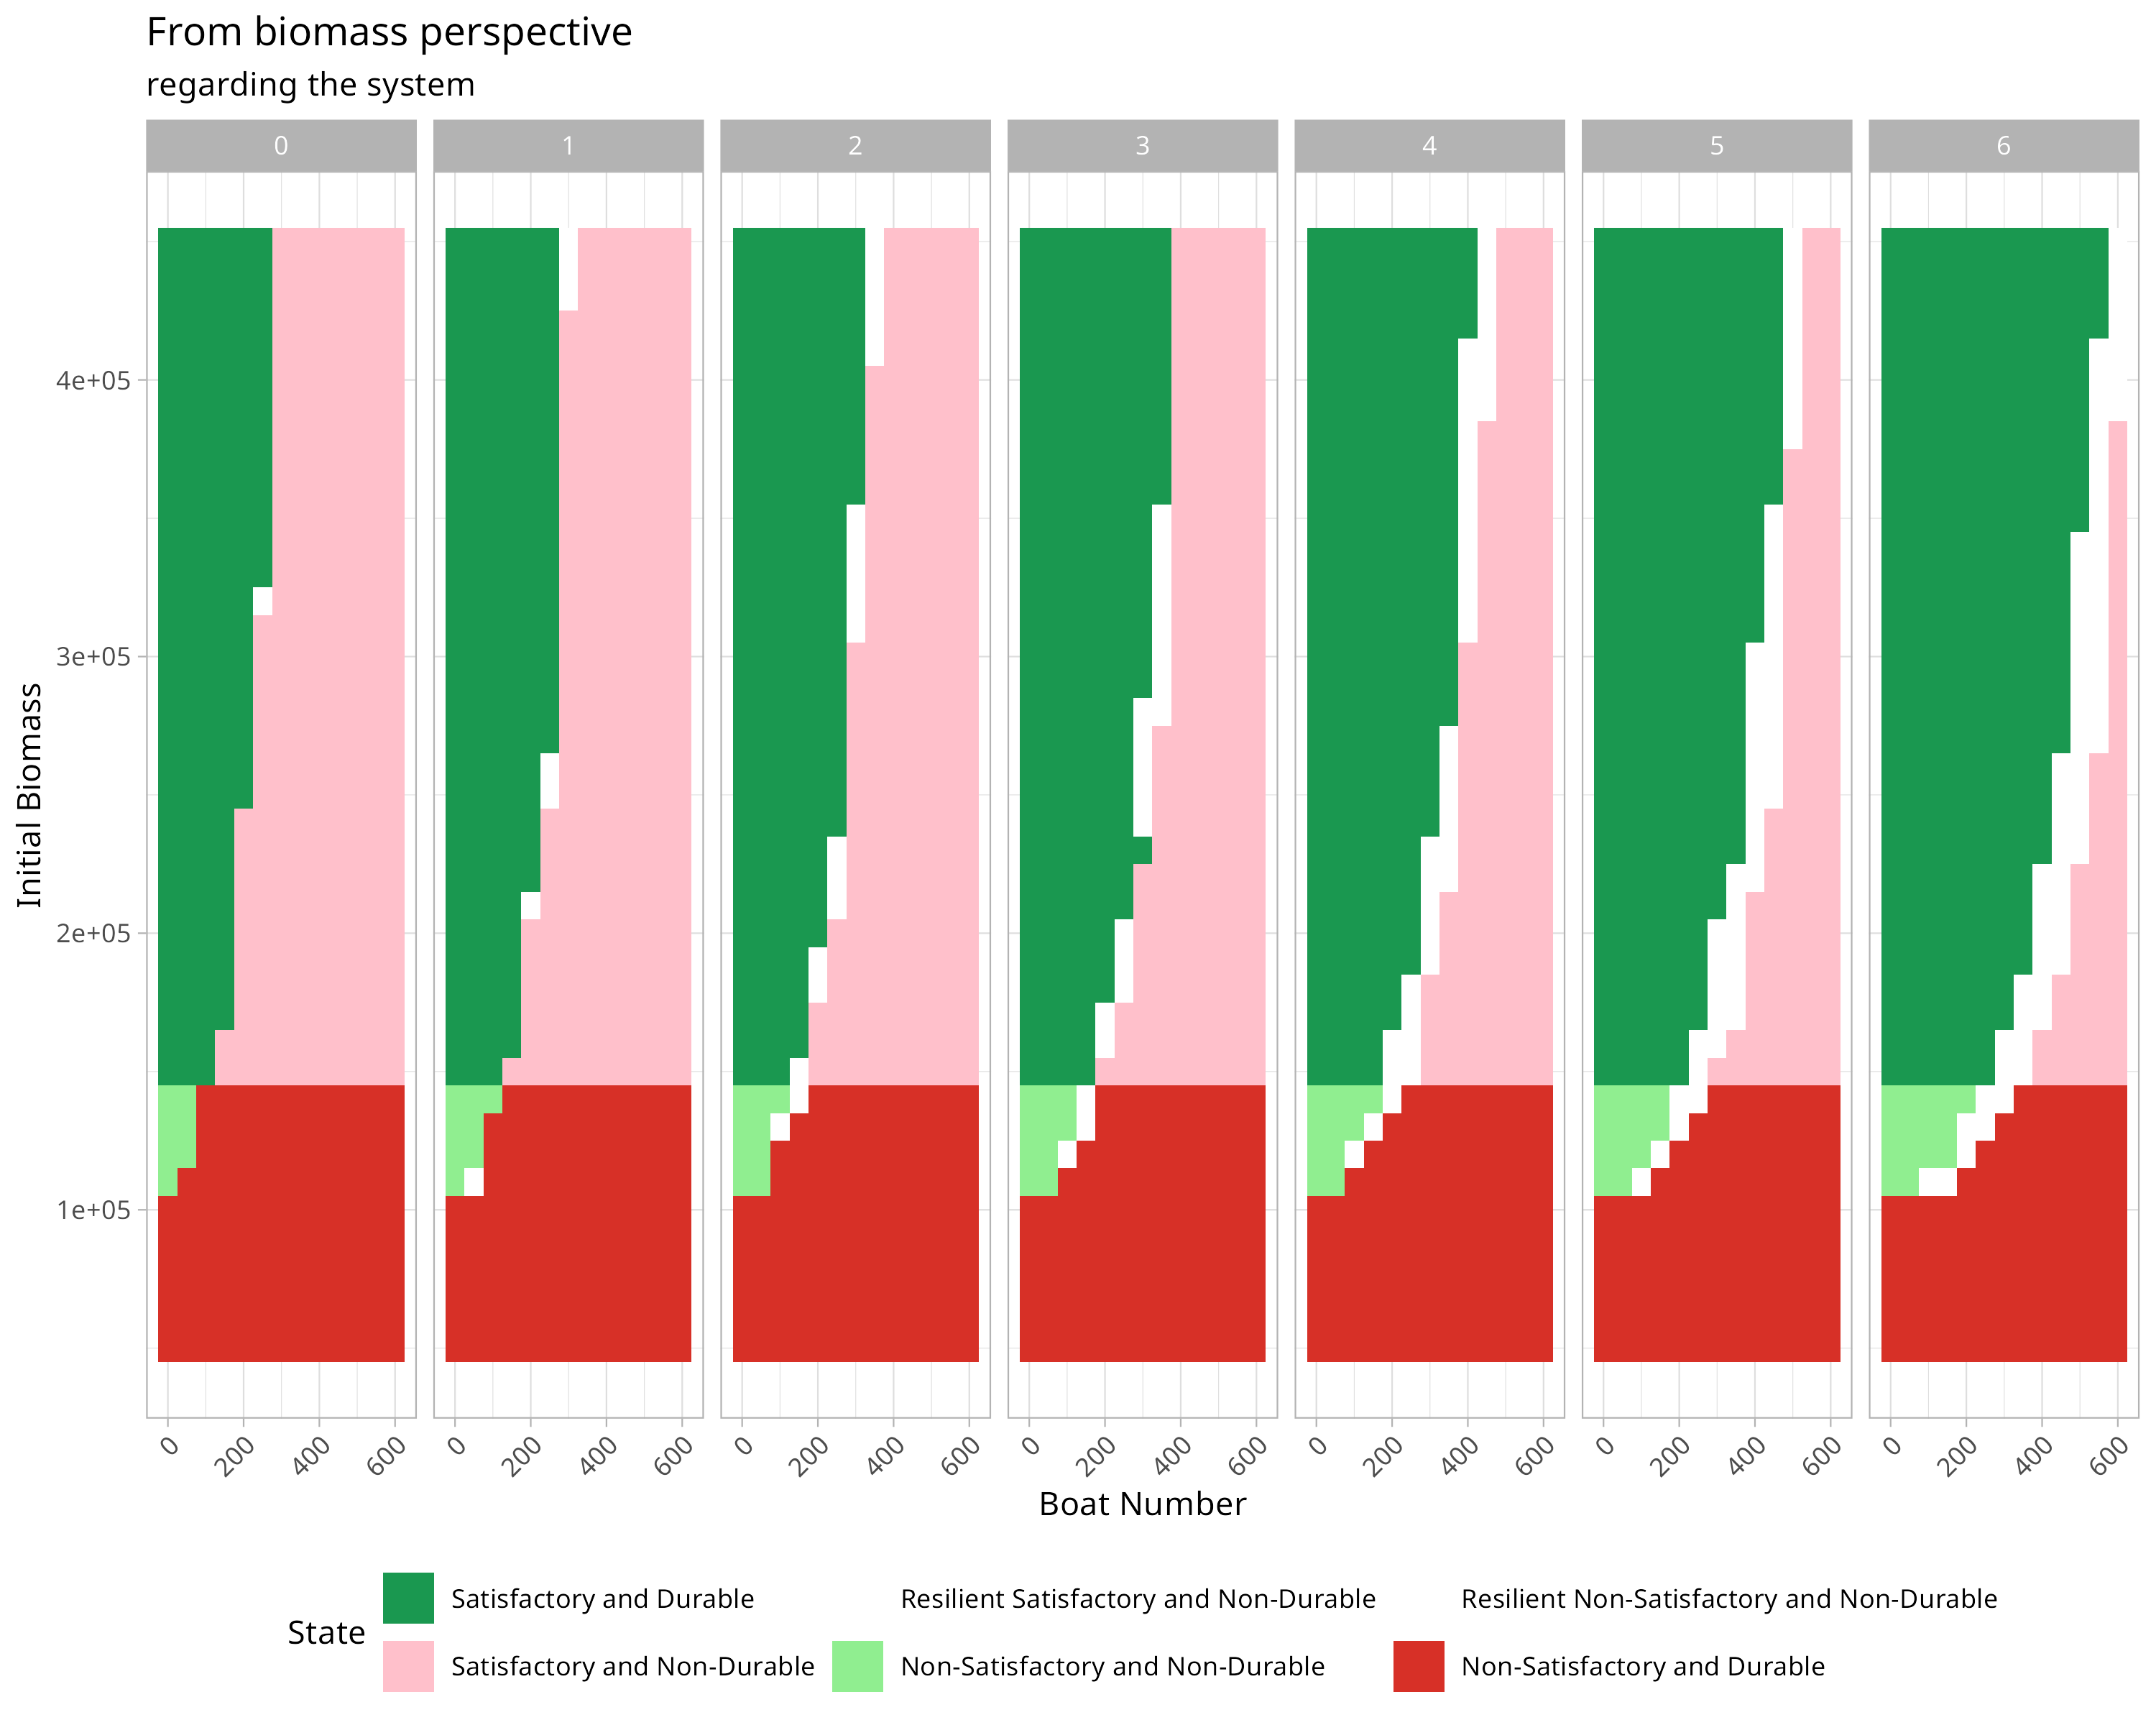
\includegraphics[width=7cm]{img/m0_pse_fatisfaction_mathias_biomass.png}
   \end{center}
\end{frame}


%-=-=-=-=-=-=-=-=-=-=-=-=-=-=-=-=-=-=-=-=-=-=-=-=
%	FRAME: ComEXp - permets de changer le point de vue
%-=-=-=-=-=-=-=-=-=-=-=-=-=-=-=-=-=-=-=-=-=-=-=-=

\section{ComExp\\ dans la pratique}

\begin{frame}[c]{Utiliser OpenMole}
  \vspace{-1cm}
  \begin{columns}[onlytextwidth,T]
    \column{\dimexpr\linewidth-30mm-5mm}
    \begin{enumerate}
        \item Initialement développé pour s'adbstraire des environnements de calcul
        \item OpenMole a pris un tournant décisif en intégrant des méthodes d'explorations complexe qui bénéficiront de l'abstraction envornomental.
    \end{enumerate}
    
    
\includegraphics[width=7.5cm]{img/OpenMOLE-Banner}
    \column{30mm}
    \begin{figure}
      
\includegraphics[width=3.4cm]{img/dragonBall.png}
    \end{figure}
  \end{columns}
\end{frame}

\begin{frame}[c]{OpenMole et Algo G.}
  \vspace{-1cm}
  \begin{columns}[onlytextwidth,T]
    \column{\dimexpr\linewidth-30mm-5mm}
    \begin{itemize}
      {\footnotesize
      \item \textbf{Méthode de calibration :}
      \begin{itemize}
        { \scriptsize
          \item Les méthodes de calibration utilisent des Algorithmes Génétiques (AG) pour explorer l’espace des paramètres.
          \item L’objectif est de trouver des ensembles de paramètres produisant des sorties pour ou plusieurs objectifs.
        }
      \end{itemize}
      
      \item \textbf{Fonctions objectifs (ou fitness) :}
      \begin{itemize}
        { \scriptsize
          \item Calculent des quantités à minimiser ou maximiser à partir des sorties du modèle.
          \item Ces fonctions quantifient la qualité des sorties du modèle en fonction des objectifs.
        }
      \end{itemize}
      
      \item \textbf{On devez définir :}
      \begin{itemize}
        {\footnotesize
          \item \textbf{Le génome du modèle :} 
          \begin{itemize}
            { \scriptsize
              \item L’AG essaiera différents génomes et conservera le meilleur découvert jusqu’alors.
              \item Sous forme de variables à minimiser.
            }
          \end{itemize}
        }
      \end{itemize}
      }
  \end{itemize}
  
    \column{30mm}
    \begin{figure}
      
\includegraphics[width=4cm]{img/tortueNJ.png}
    \end{figure}
  \end{columns}
\end{frame}

\begin{frame}[c]{OpenMole PSE}
  \vspace{-1cm}
  \begin{columns}[onlytextwidth,T]
    \column{\dimexpr\linewidth-30mm-5mm}
    
    \begin{itemize}
      \item \textbf{Objectif principal :} 
      \begin{itemize}
        { \scriptsize
          \item Explorer la diversité des sorties d’un modèle pour révéler tout son potentiel, y compris les dynamiques non anticipées.
        }
      \end{itemize}
      
      \item \textbf{Principe de base :}
      \begin{itemize}
        { \scriptsize
          \item Sélectionner des paramètres d’entrée pour produire de nouvelles valeurs de sortie.
          \item Progressivement, étendre la région couverte dans l’espace des sorties.
        }
      \end{itemize}
      
      \item \textbf{Évaluation de la rareté des sorties :}
      \begin{itemize}
        { \scriptsize
          \item L’espace des sorties est discrétisé en cellules.
          \item À chaque simulation, un compteur est incrémenté dans la cellule correspondante.
          \item Les parents associés à des cellules avec des compteurs faibles sont préférentiellement sélectionnés.
        }
      \end{itemize}
  \end{itemize}
    \column{30mm}
    \begin{figure}
      
\includegraphics[width=3.9cm]{img/the-abyss.jpg}
    \end{figure}
  \end{columns}
\end{frame}


%-=-=-=-=-=-=-=-=-=-=-=-=-=-=-=-=-=-=-=-=-=-=-=-=
%	FRAME: OLDY
%-=-=-=-=-=-=-=-=-=-=-=-=-=-=-=-=-=-=-=-=-=-=-=-=

\section{Un genre de conclusion ?}

\begin{frame}[c]{Vers des sci. transformatives ?}
  \vspace{-1cm}
  \begin{columns}[onlytextwidth,T]
    \column{\dimexpr\linewidth-30mm-5mm}
    \begin{enumerate}
        \item On retrouve évidement ici la vision des capabilités de \textsc{Sen} (1999)
        \item le lien avec la vision de l’accompagnement de \textsc{Rancière} (2003)
        \item La réduction du décalage prométhéen de \textsc{Anders} (1956) pouvoir passer a l'action
        %\item Si on accepte le fait que "l'usage est une fin en soi" $\rightarrow$ on garde une posture de domination
    \end{enumerate}
    Le processus transformatif a pour objectif de rendre libres les participants. La relation n°1 doit permettre de mesure le degré de liberté qu’on peut obtenir par l’action.
    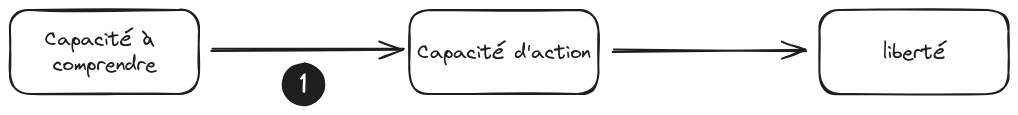
\includegraphics[width=7.5cm]{img/Drawing_jpm}
    \column{30mm}
    \begin{figure}
      
\includegraphics[width=3.9cm]{img/joker.jpg}
    \end{figure}
  \end{columns}
\end{frame}

\begin{frame}[c]{Vers des sci. transformatives}
  \vspace{-1cm}
  \begin{center}
    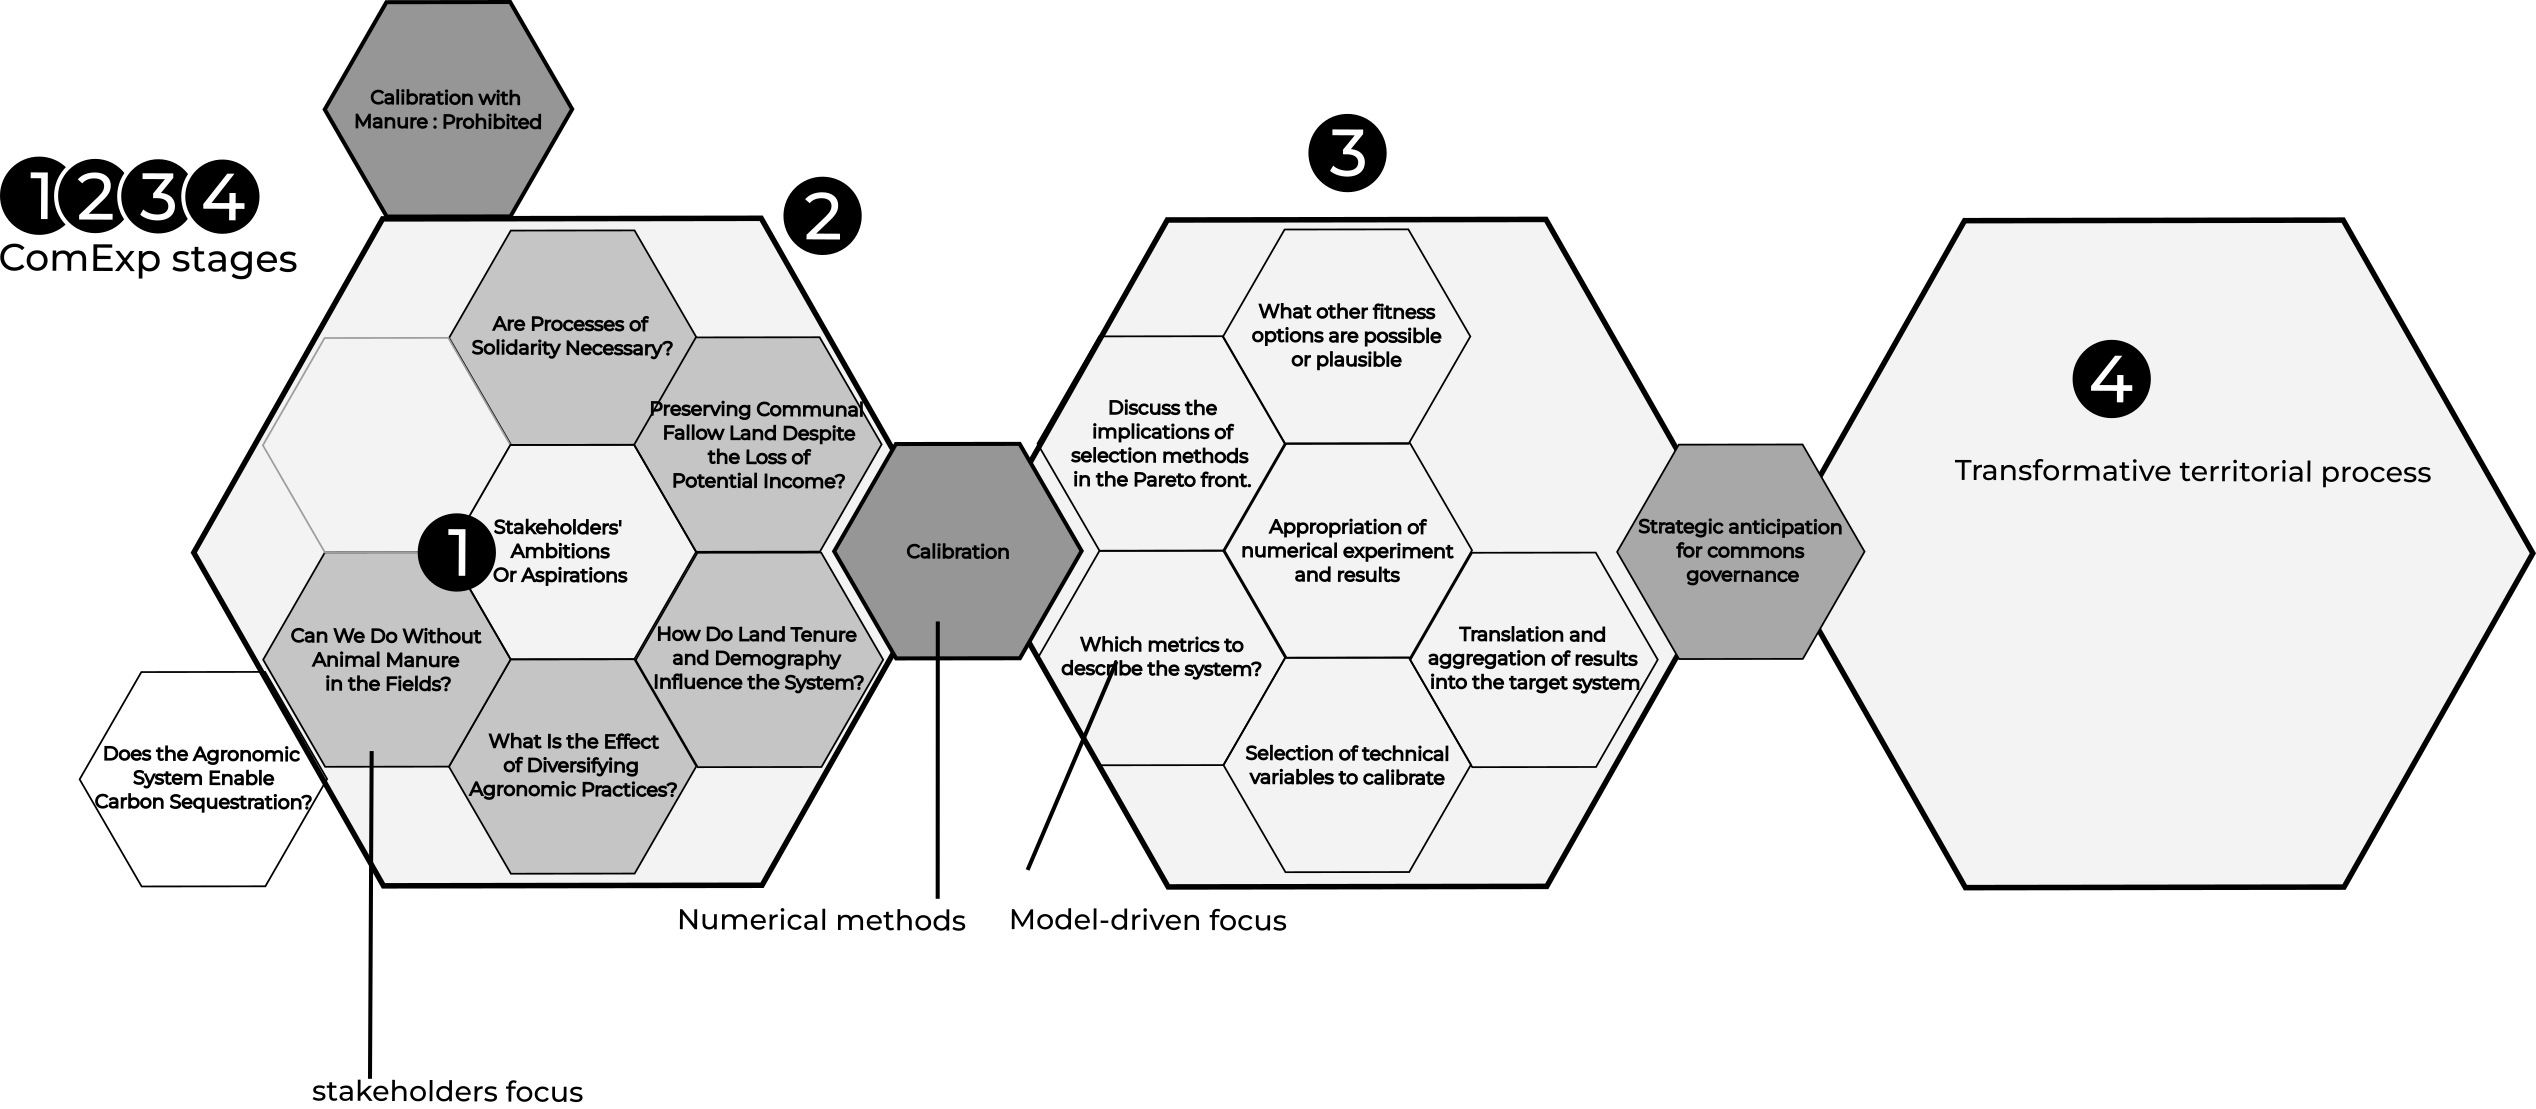
\includegraphics[width=12cm]{img/figure_discussion}
   \end{center}
\end{frame}

%-=-=-=-=-=-=-=-=-=-=-=-=-=-=-=-=-=-=-=-=-=-=-=-=
%	FRAME: MERCI DE VOTRE ATTENTION
%-=-=-=-=-=-=-=-=-=-=-=-=-=-=-=-=-=-=-=-=-=-=-=-=
{
\usebackgroundtemplate{
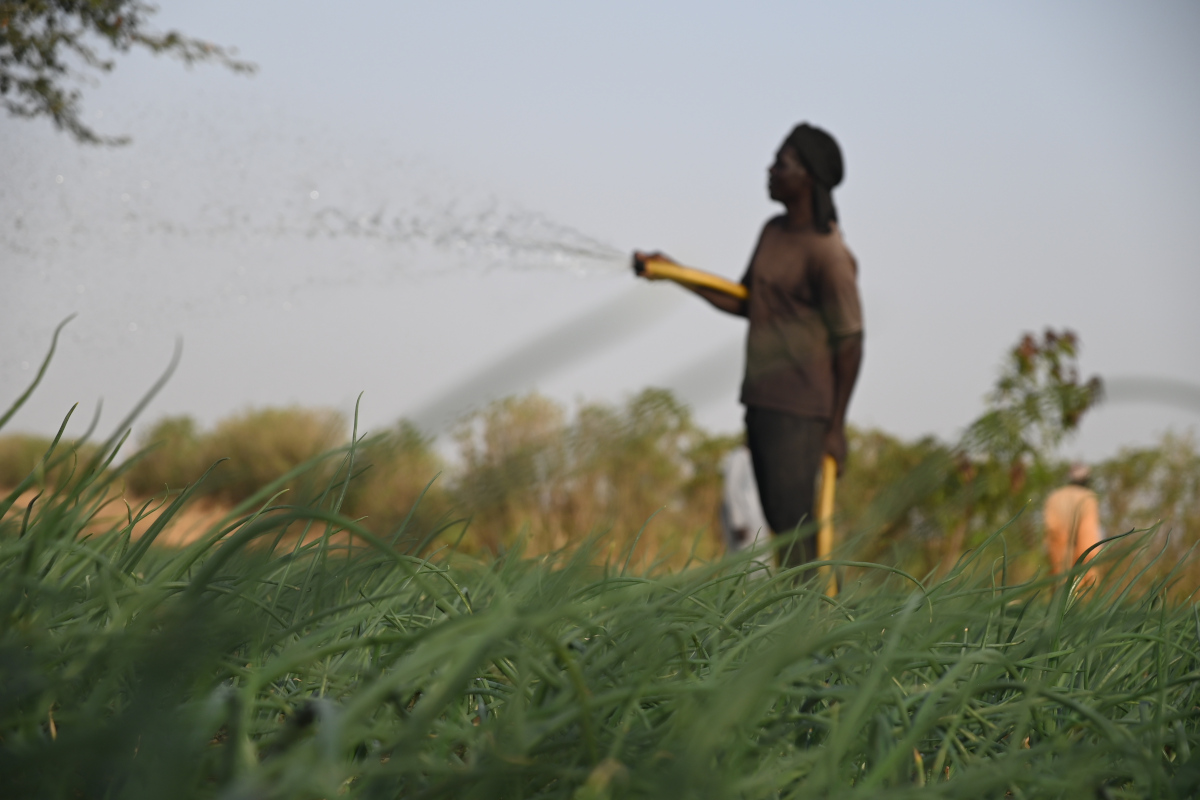
\includegraphics[width=\paperwidth]{img/arroseur_diohine.JPG}}%
\begin{frame}
  \vspace{-1em}
  \begin{minipage}[t][.8\textheight]{\textwidth}
    \color{\cnGrey}{\LARGE{Merci de votre attention}}

    \vfill

  %\hfill \small{Photo credit : Thomas m-louis. sur \includegraphics[height=0.55cm]{img/flickr_logo}}
  \end{minipage}
  \vspace{-3.5em}
  \centering
	You can find this presentation on github
\includegraphics[height=0.85cm]{img/github}

\end{frame}
}


\end{document}